\section{Implementación de Compuertas Not con Transistores}

En esta primera parte del artículo se propondrá realizar una compuerta
básica como es la inversora, o también llamada "NOT", con transistores.
Los diseños que se muestran a continuación son cuatro: dos variantes
con transistores bjt y otras dos con transistores mosfet.

\begin{figure}[H]
\begin{centering}
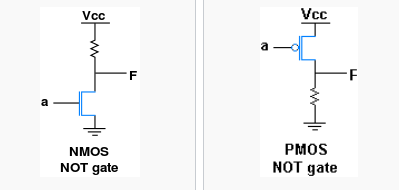
\includegraphics[scale=0.4]{mosNOT.PNG}
\qquad
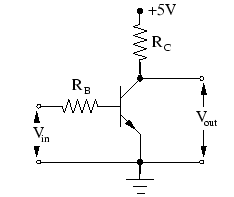
\includegraphics[scale=0.4]{npnNOT.PNG}
\qquad
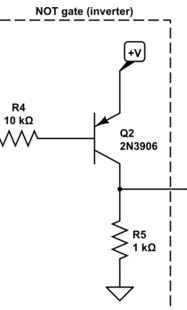
\includegraphics[scale=0.4]{pnpNOT.PNG}
\qquad
\par\end{centering}
\caption{Diseño de NOT con Transistores.}

\end{figure}

Como se muestra en las imágenes, dentro de la variante de los mosfet
se utilizó el transistor NMOS y el PMOS. En cuanto a los transistores
bipolares, se propuso un modelo con NPN y otro con PNP.

Una vez materializados estos diseños, se procedió a medir algunos
parámetros que caracterizan a la compuerta lógica. Vale aclarar que
las mediciones se realizaron solo para las compuertas con transistores
bipolares.
\vspace{5mm}
A continuación se muestran los resultados de las mediciones sin carga:
\begin{center}
\begin{table}[H]
\begin{tabular}{|c|c|c|}
\hline 
sin carga & NPN & PNP\tabularnewline
\hline 
\hline 
High-level input voltage (V) & 1 & 4,5\tabularnewline
\hline 
Low-level input voltage (V) & 0,400 & 4,2\tabularnewline
\hline 
High-level output (V) & 4,930 & 4,93\tabularnewline
\hline 
Low-level output (V) & 0,075 & 0,05\tabularnewline
\hline 
High Level Noise Margin (V) & 3,930 & 0,43\tabularnewline
\hline 
\end{tabular}\hfill    
\begin{tabular}{|c|c|c|}
\hline 
sin carga & NPN & PNP\tabularnewline
\hline 
\hline 
Low Level Noise Margin (V) & 0,325 & 4,150\tabularnewline
\hline 
Propagation delay High-Low  & 2,295 us & 140 ns\tabularnewline
\hline 
Propagation delay Low-High & 130 ns & 930 ns\tabularnewline
\hline 
Transition tiem High-Low & 1,470 us & 89 ns\tabularnewline
\hline 
Transition time Low-High & 98,500 us & 1,400 us\tabularnewline
\hline 
\end{tabular}
\caption{Mediciones - Parámetros Compuerta NOT - sin carga}
\end{table}
\end{center}

Luego se realizaron las mismas mediciones con una carga capacitiva:

\begin{center}
\begin{table}[H]
\begin{tabular}{|c|c|c|}
\hline 
con carga & NPN & PNP\tabularnewline
\hline 
\hline 
High-level input voltage (V) & 0,9 & 4,5\tabularnewline
\hline 
Low-level input voltage (V) & 0,5 & 4,2\tabularnewline
\hline 
High-level output (V) & 4,89 & 4,92\tabularnewline
\hline 
Low-level output (V) & 0,074 & 0,06\tabularnewline
\hline 
High Level Noise Margin (V) & 3,99 & 0,42\tabularnewline
\hline 
\end{tabular}\hfill
\begin{tabular}{|c|c|c|}
\hline 
con carga & NPN & PNP\tabularnewline
\hline 
\hline 
Low Level Noise Margin (V) & 0,0426 & 4,14\tabularnewline
\hline 
Propagation delay High-Low & 11,200 us & 165 ns\tabularnewline
\hline 
Propagation delay Low-High & 172,50 ns & 5,100 us\tabularnewline
\hline 
Transition tiem High-Low & 5,700 us & 164 ns\tabularnewline
\hline 
Transition time Low-High & 196 ns & 11,350 us\tabularnewline
\hline 
\end{tabular}
\caption{Mediciones - Parámetros Compuerta NOT - con carga}
\end{table}
\end{center}
Todas las mediciones se realizaron con Vcc igual a 5 Volts. En cuanto
a las mediciones de tiempo de propagación y de transición, para estas
se utilizó una excitación de onda cuadrada de 1,92 KHz.
